\chapter{Introduction Générale}
\label{chap1} 

\epigraph{<< Et au-dessus de tout homme détenant la science, il y a un savant plus docte que lui. >>}{--- \textup{Joseph, v. 76}}
%\epigraph{<< Acquire knowledge, and learn tranquility and dignity. >>}{--- \textup{Omar ibn al-Khattab}}

\NoChapterPrefix \NoChapterNumberInRef {\hypersetup{linkcolor=black} \minitoc}

%% numérotation des figures, des tables et des équations préfixé par le numéro de chapitre
\makeatletter
\renewcommand{\thefigure}{\ifnum \c@section>\z@ \thechapter.\fi
 \@arabic\c@figure}
\@addtoreset{figure}{chapter}
\makeatother

\makeatletter
\renewcommand{\thetable}{\ifnum \c@section>\z@ \thechapter.\fi
 \@arabic\c@table}
\@addtoreset{table}{chapter}
\makeatother

\makeatletter
\renewcommand{\theequation}{\ifnum \c@section>\z@ \thechapter.\fi
 \@arabic\c@equation}
\@addtoreset{equation}{chapter}
\makeatother

\newpage
\section{Contexte et problématique}
Depuis quelques années, la communauté internationale regroupant les états, les gouvernements, les associations, et les usagers s'intéresse de près  aux changements climatiques en proposant des initiatives pour limiter le réchauffement climatique. En 2015, la France a organisé à Paris la Conférence mondiale des parties à la Convention-cadre de l'ONU portant sur cette problématique, appelée aussi << COP 21 >>, où 195 pays étaient représentés. L'un des objectifs primordiaux  de cette convention est de sensibiliser les \textit{pays pollueurs} et proposer des initiatives accompagnées par des solutions durables pour réduire le réchauffement climatique lié aux gaz à effet de serre (émissions de carbone ou $CO_2$). Rester immobiles de la part de la communauté internationale et les usagers  entrainera les conséquences néfastes sur la planète comme :  \textbf{(a)} la multiplication des vagues de chaleur, \textbf{(b)} des sécheresses et des inondations, \textbf{(c)} la fonte accélérée des glaciers. 

Depuis quelques années, un nombre important d'initiatives ont été menées couvrant plusieurs secteurs comme le \textit{bâtiment} (\textit{green house}) \cite{Perez08}, \textit{l'automobile} (l'émergence des voitures électriques) \cite{Tie13}, \textit{l'électronique} \cite{Barbose13}, \textit{les réseaux sans fil} \cite{Rault14}, etc. Les expériences énergétiques menées dans ces secteurs doivent être \textit{généralisées} et \textit{capitalisées} afin de les \textit{reproduire} et les \textit{réutiliser} dans d'autres secteurs dans lesquels l'énergie électrique n'est pas complètement intégrée. Pour illustrer ces avancées, nous prenons l'exemple du secteur du bâtiment qui a connu d'énormes progrès sur la prise en compte de l'énergie. Il est intéressant de noter qu'il est parmi les plus grand consommateurs d'énergie. En France par exemple, il représente 43\% des consommations énergétiques, soit 1,1 tonne équivalent pétrole par an et par habitant\footnote{\url{http://www.logement.gouv.fr/la-politique-energetique-dans-les-batiments-2445}}. D'après les dernières statistiques, le  poste << logement >> représente à lui seul 30\% du budget des ménages. Devant cette situation, plusieurs initiatives ont été prises pour réduire cette consommation que nous proposons de classer en deux catégories principales selon la nature du bâtiment : \textbf{(i)} les initiatives pour les bâtiments \underline{existants} et \textbf{(ii)} les initiatives pour les bâtiments \underline{neufs}. Pour les bâtiments existants, les pouvoirs publics ont beaucoup communiqué afin de sensibiliser et inciter les usagers à réduire leur consommation énergétique afin qu'ils aient un comportement \underline{éco-citoyens}. Des gestes simples pourraient contribuer à cette réduction. Nous pouvons citer par exemple : \textbf{(a)} s'arranger pour que les appareils électriques fonctionnent à pleine charge, \textbf{(b)} penser aux heures creuses pour la mise en route des appareils, \textbf{(c)} acheter des  appareils ménagers en tenant compte leur niveau de consommation électrique, \textbf{(d)} limiter le plus possible le nombre d'appareils en veille, \textbf{(e)} utiliser des ampoules basse énergie. Pour une réduction maximale d'énergie, ces gestes doivent concerner tout composant électrique du bâtiment susceptible de contribuer à la réduction de la consommation énergétique.  

En ce qui concerne les initiatives pour les bâtiments neufs, l'intégration de l'énergie est prise en compte dès la conception de ce dernier. Plusieurs réglementations ont été mises en place concernant l'utilisation des matériaux et équipements plus performants et à l'utilisation des énergies. Afin d'assurer un maximum de réduction énergétique, les deux types d'initiatives doivent être combinées. Sur le plan humain, tous les acteurs de la chaîne de construction de bâtiments : les \textit{concepteurs}, les \textit{producteurs} de matériaux de construction et les \textit{usagers} doivent travailler ensemble pour assurer cet objectif. 

Revenons à notre domaine d'étude qui est l'informatique. Ce secteur avec ses composantes (matérielles et logicielles) et ses usagers participe intensivement au phénomène de réchauffement climatique. L'une des causes principales de cette situation est la demande continuelle de calcul intensif du \textit{déluge de données} générées par les contenus numériques, les applications autour des \textit{données massives} (<< Big Data >>), l'\textit{E-commerce}, et le \textit{trafic Internet}. En conséquence, les centres de données deviennent l'épine dorsale pour toute entreprise, organisme et fournisseur de stockage de données comme \textit{Amazon}, \textit{Facebook}, \textit{Google}, etc. Si nous nous référons au Conseil de Défense des Ressources Naturelles, il a indiqué que les centres de données ont consommé 91 milliards de kilowatt-heures en 2013 \cite{NRDC14b}. Ceci représente environ 3\% de la consommation d'électricité mondiale, avec un coût annuel de 9 milliards de dollars \cite{Koomey11}. Citons l'exemple du centre de données construit par \textit{Interxion}, l'installation consomme 64 mega-watts, soit l'équivalent d'une ville de 50 000 habitants\footnote{\url{http://www.interxion.com/fr/Implantations/france/paris/par7/}}. Avec la chaleur qu'ils dégagent, ils génèrent 200 millions de tonnes de gaz à effet de serre \cite{NRDC14b}; Malheureusement, pour les défenseurs de l'environnement, cette situation ne fait que s'empirer. Les experts du secteur, tels que le SMARTer 2020, rapportent que la consommation des centres de données mondiaux augmenteront de 7\% chaque année jusqu'en 2020 \cite{SMARTer12}, en raison du développement d'Internet et de l'augmentation des besoins de stockage des entreprises.

La consommation énergétique électrique de ces centres est répartie de la manière suivante : \textbf{(i)} le matériel informatique déployé sur ces centres tels que serveurs de traitement, \textbf{(ii)} le stockage et la communication, \textbf{(iii)} des équipements de refroidissement d'infrastructure (pour un kilowatt dépensé par un serveur, un autre kilowatt serait nécessaire pour le refroidir \cite{Emerson07, Tsirogiannis10}) et \textbf{(iv)} leur fonctionnement sans arrêt. \ref{fig:datacenters-energy} illustre la distribution de consommation d'énergie des équipements informatiques dans un centre de données. Nous remarquons que le processeur, la mémoire et le disque consomment la moitié d'énergie totale.

\begin{figure}
    \begin{center}
        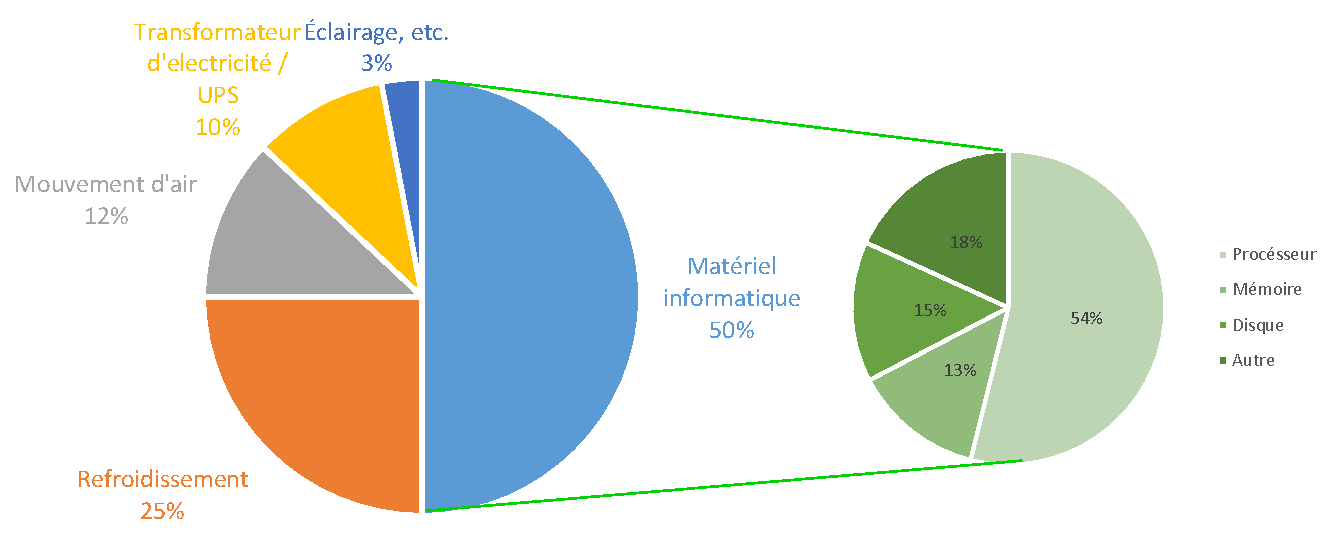
\includegraphics[scale=0.7]{chapitre1/chap1Fig/datacenters-energy.eps}
        \caption{La consommation d'énergie dans un centre de données.}
        \label{fig:datacenters-energy}
    \end{center}
\end{figure}

Face à cette situation, les industriels et les chercheurs de la communauté scientifique ne sont pas restés indifférents, ils ont pris des initiatives accompagnées de solutions réelles couvrant plusieurs actions, à savoir : \textbf{(a)} la conception de matériel avec une consommation énergétique réduite, \textbf{(b)} la restructuration des logiciels pour minimiser la consommation, \textbf{(c)} l'exploitation de divers états d'alimentation disponibles dans les nouveaux matériaux, et \textbf{(d)} une bonne conception, utilisation et contrôle de l'infrastructure des centres de données \cite{Kant09}. Ces actions ressemblent fortement à celles utilisées dans le secteur du bâtiment. Plus précisément: 
\begin{itemize}
	\item En ce qui concerne la conception de matériel avec une consommation énergétique réduite, les producteurs ont mis en place un label, appelé \textit{l'efficacité énergétique} (communément appelée PUE - power usage effectiveness) mesurant la quantité d'énergie totale consommée par un centre de données. Le consortium International Green Grid\footnote{\url{http://www.thegreengrid.org/}}, crée en 2007 et qui regroupe 501 membres et plus de 200 sociétés mondiales, vise au << verdissement >> des centres de données. L'ETSI (European Telecommunications Standards Institute) -- institut de normalisation européen des télécoms -- propose en juin 2014, une nouvelle mesure de l'efficacité énergétique comparable à celle que l'on retrouve déjà dans l'électroménager\footnote{\url{http://www.etsi.org/news-events/news/798-2014-06-press-etsi-releases-the-first-global-kpi-on-energy-efficiency-in-ict}}. Celle-ci comporte 5 niveaux de performance, du A << vert >> au I << noir >>, en passant par le G << rouge >>;
	\item En général, l'efficacité énergétique n'est pas synonyme d'efficacité de calcul \cite{Kant09}. En particulier, des techniques comme le regroupement des calculs et des transferts de données améliorent l'efficacité énergétique des logiciels. Cela est du fait qu'elles allongent les périodes d'inactivité et permettent aux dispositifs d'entrées/sorties dans des états de faible puissance. En outre, certaines opérations consomment moins d'énergie que d'autres pour un travail effectif équivalent. Il est intéressant de noter qu'une progression remarquable est constatée dans le développement de logiciels embarqués économiques. Cependant, il manque encore un travail considérable en terme  méthodologique, conceptuel, et validation pour le développement de logiciels économiques de tout bord \cite{Kant09}.
	\item De nos jours, presque tous les principaux composants d'un serveur offrent des modes de contrôle d'énergie. Ils se matérialisent sous forme d'états de puissance : une collection de modes opérationnels qui compromettent la consommation d'énergie pour la performance. Un état de puissance pour un composant est dit \textit{actif} si celui-ci reste opérationnel dans cet état, sinon l'état est dit \textit{inactif}. L'ACPI (\textit{Advanced Configuration and Power Interface}) fournit une nomenclature standard pour ces états et définit également les interfaces logicielles pour les gérer. L'ACPI est implémentée dans tous les principaux systèmes d'exploitation (\acrshort[hyper=false]{SE}) sous forme de la gestion de l'alimentation dirigée par le SE\footnote{\url{http://www.uefi.org/sites/default/files/resources/ACPI_6_1.pdf}}.
	\item Plusieurs technologies sont actuellement envisagées pour rendre l'infrastructure d'un centre de données plus efficace. Par exemple, la plupart des serveurs fonctionnent à une utilisation relativement faible la plupart du temps. Cependant, une double alimentation redondante (PSU) est souvent utilisée pour la fiabilité, ce qui se traduit par une charge et une efficacité relativement faible. Pour les infrastructures de refroidissement; dans une démonstration de concept d'un centre de données exploité par Intel, le refroidissement ambiant avec un échange d'air jusqu'à 32° a été utilisé. Le résultat obtenu est une économie de 67\% de puissance avec un refroidissement ambiant 91\% du temps \cite{Atwood08}. En descendant la hiérarchie, des solutions de refroidissement plus intelligentes ont émergé au niveau du châssis, des enceintes et du serveur sous la forme de ventilateurs à vitesse variable modulés par des mesures de température \cite{Kant09}.
\end{itemize}

La discussion ci-dessous que nous avons initiée concerne le domaine informatique d'une manière générale. Nous nous focalisons sur un de ses postes importants à savoir les systèmes de gestion de données (\acrshort[hyper=false]{SGBD}), ou les systèmes de stockage de donnée hébergés par les centres de données. Ceci représente le contexte de cette thèse. Les SGBD sont les plus gros consommateurs d'énergie électrique. Cela est dû au fait qu'ils effectuent des opérations (jointure, union, agrégation, etc. ), impliquant des tables ou des structures de données volumineuses qui nécessitent toutes les ressources d'un centre de données (CPU, mémoire, et  réseau). 

Devant cette situation critique, deux articles de vision ont été publiés par des chercheurs de la \textit{communauté de bases de données} provenant à la fois du milieu académique (Stavros Harizopoulos et al. \cite{Harizopoulos09} de MIT) et industriel (Goetz Graefe \cite{Graefe08} de HP). Ils ont mis l'accent sur l'intégration de l'énergie dans la conception et l'exploitation des bases de données. Les recommandations de ces auteurs coïncident avec ce que la communauté scientifique a identifié, à savoir l'utilisation des matériels et logiciels économiques \cite{PoessN08}. Les SGBD peuvent bénéficier des matériels économiques existants (comme les supports de stockage amovible \cite{Schall10}, les cartes graphiques \cite{Hurson16}, etc.).  

\begin{figure}
	\begin{center}
		\includegraphics[scale=0.5]{chapitre1/chap1Fig/composantesSGBD.png}
		\caption{Les composantes principales d'un SGBD}
		\label{fig:composantesSGBD}
	\end{center}
\end{figure}

Rappelons que la consommation énergétique d'un SGBD dépend de la base de données qu'il héberge. Plus précisément, elle dépend de son schéma (le nombre de tables et les attributs), sa population (en termes d'instances) et son exploitation via des requêtes. La plus grosse consommation d'un SGBD est due au calcul effectué par ses composantes principales : l'optimiseur de requêtes, le gestionnaire de buffer, le contrôleur de concurrence, le gestionnaire des méthodes d'accès, le gestionnaire de stockage, etc. comme le montre la \ref{fig:composantesSGBD}. Les travaux existants sur l'incorporation de la dimension << énergie >> se focalise sur la partie traitement de requêtes. Ils supposent que la base de données est déjà conçue et déployée sur un SGBD. L'optimisation de requêtes dans les bases de données est une tâche difficile, et souvent modélisée comme un problème d'optimisation à base de contraintes. Ces dernières représentent plusieurs besoins non-fonctionnels comme le temps de réponse, le coût de stockage, le coût de maintenance. Les approches proposées pour résoudre cette problématique font souvent appel au développement de modèles de coût mathématiques estimant le ou les besoins non-fonctionnels utilisés. Les premiers travaux sur l'incorporation de l'énergie dans le monde des bases de données (côté logiciel) étaient le développement de modèles de coût mathématiques estimant la consommation énergétique lors de l'exécution de requêtes. Ces modèles prennent en compte des paramètres couvrant plusieurs entités logicielles et matérielles de la base de données cible tels que son schéma (par ex. la taille des tables, la longueur de tuples, etc.), la charge de requêtes (par ex. le type de requêtes, les facteurs de sélectivité des jointures et des prédicats de sélections, tailles des résultats intermédiaires, etc.), le matériel (par ex. la taille de tampon, la taille de page du disque, etc.) et la plate-forme de déploiement (par ex. RAM, la taille du disque, le nombre de nœuds, etc.).

D'autres efforts ont été effectués dans le développement des bancs d'essai permettant aux chercheurs de tester l'efficacité de leurs modèles économiques dédiés à la gestion de la base. Nous pouvons citer l'exemple du banc d'essai TPC-Energy \cite{TPCE} lancé en 2007. 

L'ensemble de ces travaux suppose que la base de données est déjà déployée et s'intéresse particulièrement à la partie optimisation de requêtes effectuée par le SGBD hébergeant cette base. Or, d'autres phases de cycle de vie de la base de données peuvent être sensibles à l'énergie comme la phase physique -- souvent associée à l'image de la qualité et de performance de toute base de données -- dans la quelle des structures d'optimisation comme les index, les vues matérialisées, le partitionnement doivent être sélectionnées. Ces structures sont souvent utilisées par les optimiseurs de requêtes pour finir des plans efficaces (\ref{fig:cyclehors}).

\begin{figure}
	\begin{center}
		\includegraphics[scale=0.5]{chapitre1/chap1Fig/cyclehors.pdf}
		\caption{L'énergie dans le cycle de vie de conception de base de données}
		\label{fig:cyclehors}
	\end{center}
\end{figure}

Dans cette thèse, nous tenterons à répondre à ces limites en proposant des modèles mathématiques plus robustes pour estimer l'énergie et proposer une démarche de conception physique dirigée par la consommation énergétique. 

Dans les sections suivantes, nous présentons les objectifs de notre thèse et l'ensemble de contributions réalisées.

\section{Objectifs et contributions}
Notre premier objectif est de sensibiliser les usagers et les concepteurs de bases de données de la dimension énergétique, en suivant l'expérience du domaine du bâtiment, en proposant des solutions pour des bases de données déjà existantes. Cela doit passer par la revisite des travaux sur l'optimisation de requêtes, considérée comme un poste gourmand en énergie. L'intégration de l'énergie dans les optimiseurs de requêtes peut se faire en suivant plusieurs scénario : (i) les optimiseurs de requêtes dirigées par seulement l'énergie, (ii) les optimiseurs de requêtes dirigées par plusieurs besoins non-fonctionnels y compris l'énergie. Dans la continuité de la reproduction des efforts du secteur du bâtiment, nous avons déployé nos solutions énergétiques sur un SGBD open source (PostgreSQL) afin de valider nos résultats et surtout pour sensibiliser et motiver les usagers et les concepteurs pour intégrer cette dimension dans leurs solutions. 
Le second objectif est de pousser plus loin notre réflexion sur la conception verte des bases de données, et l'appliquer sur une autre phase de cycle de vie qui est la phase physique. 

Afin de répondre à nos objectifs, nous nous sommes fixées un ensemble d'actions qui sont : 
\begin{enumerate}
	\item \textit{Un audit sur les composants d'un SGBD.} Pour économiser l'énergie, il faut d'abord identifier les postes sensibles. Cela est établi par un audit de l'ensemble de composants d'un SGBD (\ref{fig:composantesSGBD}). Dans un serveur informatique, il y a généralement cinq consommateurs d'énergie, à savoir, le processeur, les disques, la mémoire, les dispositifs d'entrées/sorties (\acrshort[hyper=false]{E/S}) et la carte mère. Il faut étudier le comportement du système lors de l'exécution d'une requête par le SGBD et son impact sur l'énergie. Atteindre une efficacité énergétique nécessite des améliorations dans le profil de la consommation d'énergie de chaque composant du système.
	\item \textit{L'adoption dynamique de composants matériels.} L'adoption de composants matériels dynamiquement pourrait aider à améliorer l'efficacité énergétique. Par exemple, l'exécution du processeur à une fréquence inférieure permet de réduire la tension, résultant d'une économie d'énergie. Cette technique, qui met en œuvre un compromis entre la performance et l'énergie, est connue comme l'ajustement dynamique de la tension et de la fréquence (\acrshort[hyper=false]{DVFS}), la tension et la fréquence sont ajustées à la volée. Une technique similaire existe pour les disques et mémoires vivres \cite{Sjalander14}.
	En outre, en employant des lecteurs de disques \gls{SSD}, des cartes graphiques puissantes pour le traitement, une grande configuration de mémoire, processeurs et mémoires de faible consommation ont pourrait diminuer la consommation d'énergie totale du système.
	Intégrer ces techniques directement dans l'SGBD afin de contrôler son bon fonctionnement est nécessaire, car le SGBD a la connaissance sur la donnée. 
	\item \textit{Le développement des modèles de coût mathématiques}. Toute prise de décision d'un SGBD est souvent orchestrée par un modèle  de coût mathématique estimant un besoin non-fonctionnel. Dans le contexte de l'energie, l'optimiseur de requêtes doit être associé à des modèles de coût robustes qui doivent prendre en compte tous des paramètres pertinents des composantes sensibles à l'énergie électrique. 
	\item \textit{Vers une sélection des structures d'optimisation vertes}. Les structures d'optimisation  (les vues matérialisées, les index, etc.) qui ont émergé avec l'arrivée des entrepôts de données sont souvent sélectionnées avec des algorithmes dirigés par des modèles de coût mathématiques, estimant la performance de requêtes ou le coût de maintenance. Cette sélection doit être revisitée pour intégrer le coût énergétique. 
\end{enumerate}
Dans cette thèse nous considérons les actions (1), (3) et (4). L'action (2) n'est pas considéré dans notre étude pour plusieurs raisons :
\begin{itemize}
	\item Les techniques basées sur le matériel requièrent de nouveaux matériels, car d'une part les nouvelles technologies comme le DVFS ne sont pas disponibles sur tout les processeurs et d'autre part les nouveaux disques SSD sont très cher et ont un problème de durée de vie. 
	\item Il existe diverses gammes pour chaque composant matériel, donc développer des méthodes sur une seule gamme ou marque limite la portabilité de ces méthodes.
	\item Les techniques logicielles sont préférées dans le contexte des bases de données car le SGBD a une connaissance détaillée sur les charges de requêtes, les plans d'exécution, les informations sur les données, etc.
\end{itemize}

Pour répondre aux limitations précédentes, nos principales contributions, décrites dans cette thèse, sont les suivantes :
\begin{description}
	\item[La proposition d'un modèle de coût énergétique pour des requêtes isolées.] Pour exécuter une requête \acrshort[hyper=false]{SQL}, l'optimiseur doit sélectionner son meilleur plan d'exécution qui peut être représenté par un arbre d'opérations algébriques correspondant à cette requête. Une fois identifié, l'optimiseur exécute ce plan étape par étape\footnote{Ce mode d'exécution est appelé le mode itérateur.}. Le mode d'exécution des requêtes influence la puissance électrique consommée et l'énergie totale. Cette observation est complètement ignorée par les travaux de l'état de l'art lors de la définition des modèles de coût. Ce dernier doit prendre en considération la relation entre les paramètres du modèle (linéaire, logarithmique, exponentielle. etc.) pour avoir des résultats fiables. Les travaux existants supposent que cette relation est linéaire. Dans cette thèse, nous avons montré que la relation est non-linéaire. 
	
	\item[Modèle de coût énergétique pour des requêtes concurrentes.] Dans un environnement réel des centres de données, le SGBD exécute un ensemble de requêtes simultanément de façon concurrente. Cette hypothèse n'est pas prise en compte par les travaux existants lors de la définition des modèles de coût. En conséquence, nous avons  étendu notre modèle de coût pour prendre en charge ce scénario. Cela est utile pour plusieurs tâches telles que le contrôle d'admission, l'ordonnancement des requêtes et le contrôle d'exécution des requêtes avec l'objectif d'améliorer l'efficacité énergétique.  
	
	\item[Traitement de requêtes éco-énergétique.] Avec la présence de modèle de coût, nous proposons une  méthodologie qui intègre l'énergie dans le processus de traitement des requêtes pour produire des plans d'exécutions réduisant leur consommation. Cette démarche a été implémentée sous le SGBD PostgreSQL.
	
	\item[Conception physique éco-énergétique.] Nous avons proposé une approche de sélection de structures d'optimisation en prenant en compte plusieurs besoins non-fonctionnels : la performance de requêtes, l'espace de stockage et la consommation énergétique. Nous avons choisi le cas des vues matérialisées; considérées comme des structures redondantes du fait qu'elles exigent une espace de stockage et un coût de maintenance. Nous avons alors formalisé le problème de sélection des vues matérialisées comme un problème multi-objectif et nous avons proposé des algorithmes avancés pour sa résolution.                     
	 \end{description}

\section{Organisation de la thèse}

% TODO: update graph, use Fig1.3 of Beloglazov11 thesis
\begin{figure}
	\begin{center}
		\includegraphics[scale=0.7]{chapitre1/chap1Fig/chapters-org2.pdf}
		\caption{La répartition des chapitres de la thèse.}\label{fig:chapitres}
	\end{center}
\end{figure} 

D'un point de vue organisationnel, le reste de la thèse s'articule autour de six chapitres.

Dans le \ref{chap2}, nous présentons un état de l'art sur le cycle de vie de conception des bases de données avancées, avec une focalisation particulière sur la phase physique. Le chapitre décrit aussi le module de traitement de requêtes dans un SGBD relationnel et propose la conception d'un optimiseur de requêtes éco-énergétique. Le chapitre cite également les techniques d'optimisations multi-objectifs et les solutions proposées dans le contexte des bases de données pour sa résolution.

Dans le \ref{chap3}, nous présentons un état de l'art sur les différentes techniques d'amélioration de l'efficacité énergétique dans les systèmes informatiques en général, et dans les bases de données en particulier, les différents concepts requis pour ce travail ainsi que les notions de bases sur l'énergie et les modèles de coût proposés sont présentés.

Dans le \ref{chap4}, nous étudions le comportement de l'énergie des bases de données sur le matériel informatique. Il s'agit d'identifier les paramètres et ses caractéristiques liées à la consommation énergétique des requêtes. A la base de cette étude empirique, nous proposons un modèle de coût pour estimer la consommation énergétique d'une requête SQL isolée. Ensuite, le cas des requêtes exécutées simultanément de façon concurrente est étudié. Nous étendons le modèle coût pour une seule requête vers une charge de requêtes, et nous adaptons les paramètres et les algorithmes pour avoir une meilleure estimation. Nous validons notre modèle sur une variété de configurations logicielles et matérielles. 

Dans le \ref{chap5}, nous étudions le cas de traitement des requêtes dans un SGBD relationnel, afin de savoir l'impact de chaque phase de ce traitement sur la consommation d'énergie du système. Suivant cette étude, nous proposons une méthodologie qui intègre l'énergie dans le processus de traitement des requêtes pour produire des plans d'exécutions réduisant la dissipation d'énergie.

Le \ref{chap6} aborde le problème d'intégration de l'énergie dans la phase de conception physique des bases de données. L'analyse est effectuée en prenant le cas des vues matérialisées. Une formalisation multi-objectif est proposée, et un algorithme évolutionnaire est utilisé pour résoudre le problème de sélection des vues matérialisées.

En fin, nous concluons la thèse par un bilan général sur nos contributions, et l'évocation des perspectives qui s'offrent à l'issue de notre travail dans le \ref{chap7}.

Ce mémoire comprend également trois annexes. L'\ref{annex:CostModelEstimations} décrit le processus d'estimation des coûts dans la phase d'optimisation des requêtes dans un SGBD. Elle donne les fonctions d'estimation de cardinalité des résultats intermédiaires, et détaille les formules d'estimation du coût d'entrées/sorties des opérateurs physiques. L'\ref{annex:ConfidenceBounds} étudie les bornes de confiance dans les données et les résultats de modèle de coût énergétique afin de confirmer la qualité de la modélisation. L'\ref{annex:TrainQueries} liste les requêtes utilisées pour construire le modèle de coût énergétique lors de la phase d'apprentissage.

Les principales contributions de notre thèse sont réparties dans les Chapitres \ref{chap4}, \ref{chap5} et \ref{chap6}. La \ref{fig:chapitres} schématise les grands axes de ce travail et leur répartition dans chaque chapitre.
Chacun des ces chapitres a donné lieu à un ensemble de communications et de publications dans des conférences internationales :

\textbf{Publications internationales :}

\begin{quote}
	\cite{Roukh17} 
	\textbf{Amine ROUKH}, Ladjel BELLATRECHE, Selma BOUARAR, Ahcène BOUKORCA : Eco-Physic: Eco-Physical Design Initiative for Very Large Databases. Information Systems. Elsevier, 2017. \href{http://dx.doi.org/10.1016/j.is.2017.01.003}{\textsc{[doi]}}.
\end{quote}

\textbf{Communications internationales :}

\begin{quote}
	\cite{Roukh15a} \textbf{Amine ROUKH}, Ladjel BELLATRECHE : Eco-Processing of OLAP Complex Queries. In proceedings of 17th International Conference on Big Data Analytics and Knowledge Discovery (DAWAK). LNCS, Springer, Valencia, Spain, September 1-4, 2015. p. 229-242. \href{http://dx.doi.org/10.1007/978-3-319-22729-0_18}{\textsc{[doi]}}.                                                                                                                                                                                                                                                                               \end{quote} 

\begin{quote}
	\cite{Roukh15b} \textbf{Amine ROUKH} : Estimating Power Consumption of Batch Query Workloads. In proceedings of 5th International Conference Model and Data Engineering. Springer International Publishing (MEDI), Rhodes, Greece, September 26-28, 2015. p. 198-212. \href{http://dx.doi.org/10.1007/978-3-319-23781-7_16}{\textsc{[doi]}}.
\end{quote}

\begin{quote}
	\cite{Roukh15c} 
	\textbf{Amine ROUKH}, Ladjel BELLATRECHE, Ahcène BOUKORCA, Selma BOUARAR : Eco-DMW: Eco-Design Methodology for Data Warehouses.  In proceedings of 15th International Workshop on Data Warehousing and OLAP (DOLAP). ACM, Melbourne, Australia, October 23 - 23, 2015. p. 1-10. \href{http://dx.doi.org/10.1145/2811222.2811230}{\textsc{[doi]}}. 
\end{quote}

\begin{quote}
	\cite{Roukh16a} \textbf{Amine ROUKH}, Ladjel BELLATRECHE, Carlos ORDONEZ : EnerQuery: Energy-Aware Query Processing.  In proceedings of 16th International on Conference on Information and Knowledge Management (CIKM). ACM, Indianapolis, Indiana, USA — October 24 - 28, 2016. p. 2465-2468. \href{http://doi.acm.org/10.1145/2983323.2983334}{\textsc{[doi]}}.
\end{quote}

\begin{quote}
	\cite{Roukh16b} \textbf{Amine ROUKH}, Ladjel BELLATRECHE, Nikos TZIRITAS, Carlos ORDONEZ : Energy-Aware Query Processing on Parallel Database Cluster Nodes. In proceedings of 16th International Conference on Algorithms and Architectures for Parallel Processing (ICA3PP). Springer International Publishing, Granada, Spain, December 14-16, 2016. p. 260-269. \href{http://dx.doi.org/10.1007/978-3-319-49583-5_20}{\textsc{[doi]}}.
\end{quote}

\begin{quote}
	\cite{Ouared16} Abdelkader OUARED, Yassine OUHAMMOU, \textbf{Amine ROUKH} : A Meta-advisor Repository for Database Physical Design. In proceedings of 6th International Conference on Model and Data Engineering (MEDI) Springer International Publishing, Almería, Spain, September 21-23, 2016. p. 72-87. \href{http://dx.doi.org/10.1007/978-3-319-45547-1_6}{\textsc{[doi]}}.
\end{quote}

\begin{quote}
	\cite{Bouarar17} Selma BOUARAR, Ladjel BELLATRECHE, \textbf{Amine ROUKH} : Eco-Data Warehouse Design Through Logical Variability. In proceedings of 43rd International Conference on Current Trends in Theory and Practice of Informatics (SOFSEM). Springer International Publishing, Limerick, Ireland, January 16-20, 2017. p. 436-449. \href{http://dx.doi.org/10.1007/978-3-319-51963-0_34}{\textsc{[doi]}}.
\end{quote}

% La répartition des publications et des communications à travers nos chapitres est la suivante :
% \begin{itemize}
% 	%\item Chapitre 3 : \cite{}.
% 	\item Chapitre 4 : \cite{Roukh15a, Roukh15b}.
% 	\item Chapitre 5 : \cite{Roukh16a, Roukh16b}.
% 	\item Chapitre 6 : \cite{Roukh15c}.
% 	%\item Chapitre 6 : \cite{}.
% \end{itemize}